\documentclass[a4paper]{article}
\usepackage[margin=1.5cm]{geometry} % Change the margins
\usepackage[utf8]{inputenc} % - Defines what coding LaTeX uses. Use this one.
\usepackage[english]{babel}
\usepackage[T1]{fontenc}
\usepackage{graphicx} % - Package for including images in the document.
\usepackage{amsmath}
\usepackage{mathtools}
\usepackage{textgreek}
\usepackage{caption} % Correct spacing for captions
\usepackage{siunitx} % Package for handling numbers (ex \num{1e6}), units (ex \SI{15,3}{Nm}) and intervals (ex \SIrange{10}{20}{\celcius}) correctly
\sisetup{output-decimal-marker={,},range-phrase=--,range-units=single,exponent-product=\cdot} % If you write in English, remove output-marker...
\graphicspath{ {Images/} } % - Path to where the images are located on your computer. In this case I have a folder (look to the left) "Images" where the images are gathered.
\usepackage{hyperref} % - Package for including hyperlinks in the document.
\usepackage[style=apa,backend=biber]{biblatex} % APA-referenser
\usepackage{mhchem}
\DeclareLanguageMapping{swedish}{swedish-apa}  % APA-referenser
 % - Package for the bibliography ("referenser").
\addbibresource{references.bib} % - From where, i.e. which file, the references are taken. The bibliography file is called name.bib; see left column.

\title{Lab 1}

\author{
Author \\
{Klas Mannberg,   klaman-8@student.ltu.se
} \\ \\

\includegraphics[width=0.2\textwidth]{ltu_swe.jpg}}
\date{16 April 2020}

\begin{document}

\maketitle

\section{Exercies}
\subsection{Exercise 1}
In figure \ref{fig:1} we see the first sinusoid with the function $x(t) = 2 \cdot sin(2 \cdot \pi \cdot 3 \cdot t+\pi/3)$ as a solid blue line. The second sinusoid is shown as a red dashed line representing the function $y(t) = 2 \cdot sin(2 \cdot \pi \cdot t)$.
\begin{figure}
    \centering
    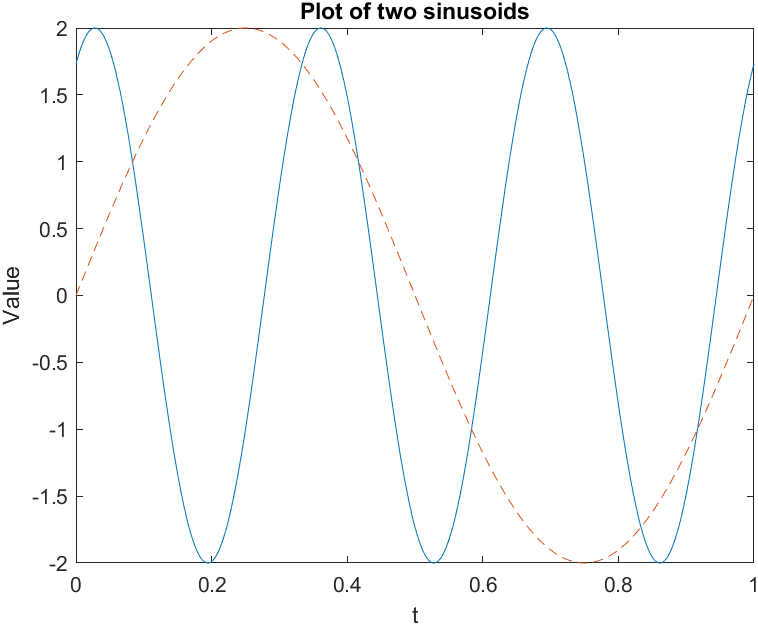
\includegraphics[width=0.6\textwidth]{1.png}
    \caption{Exercise 1, plot of two sinusoids}
    \label{fig:1}
\end{figure}

\subsection{Exercise 2}
Signals given:
\begin{itemize}
    \item $x(t) = cos(6 \cdot \pi \cdot t)$ \\
    \item $y(t) = |t|^{1/3}$ \\
    \item $z(t) = x(t)y(t)$ \\
\end{itemize}
The signals $\{x(t),y(t),z(t)\}$ are plotted in picture \ref{fig:2} as separate figures.
\begin{figure}
    \centering
    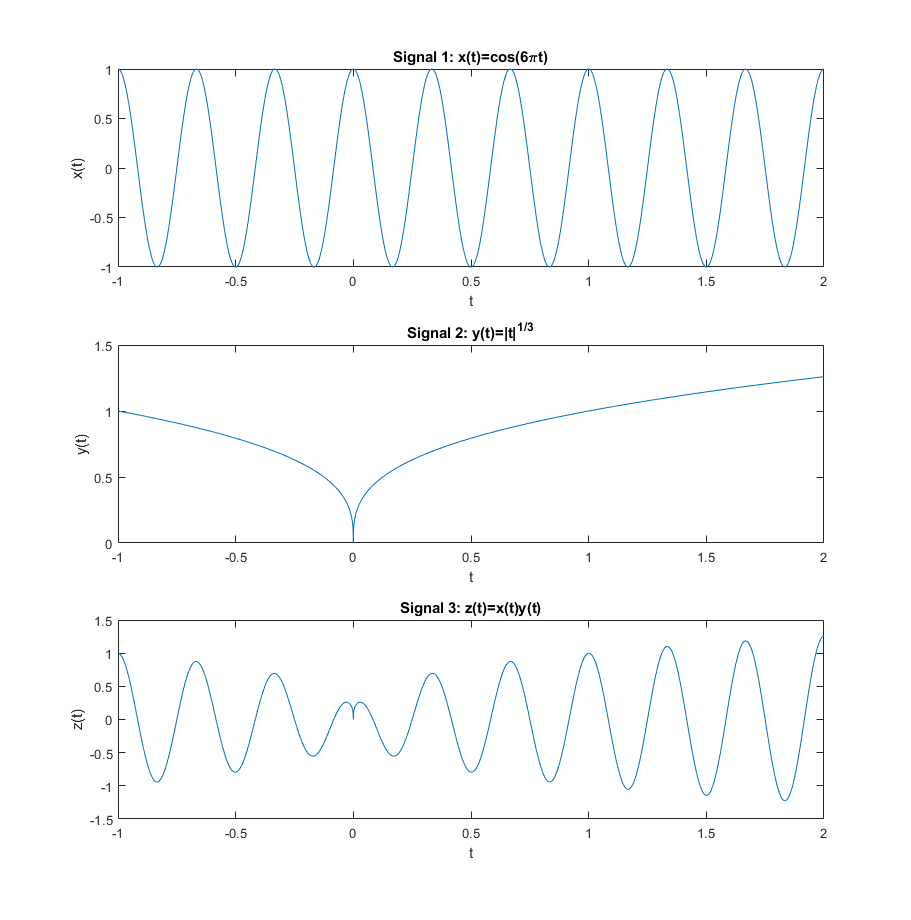
\includegraphics[width=0.6\textwidth]{2.png}
    \caption{Exercise 2, plot of three signals}
    \label{fig:2}
\end{figure}
\subsection{Exercise 3}
The three new samples of $\{x(t),y(t),z(t)\}$, $\{x[t T_s],y[t T_s],z[t T_s]\}$ are shown in picture \ref{fig:3}.
\begin{figure}
    \centering
    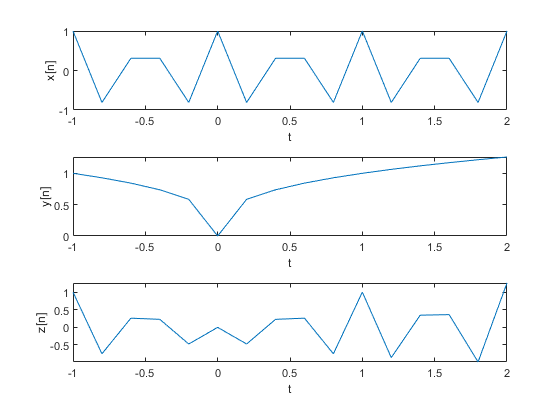
\includegraphics[width=0.6\textwidth]{3.png}
    \caption{Exercise 3, plot of three samplings of signals}
    \label{fig:3}
\end{figure}
\subsection{Exercise 4}
If we insert an impulse $x = \delta$ the impulse response would equal $\frac{1}{8}=0.125$ when $n-k=0$ for $\delta[n-k]$. Looking at the equation itself we can clearly see that $n-k=0$ for $n=0,1,2,..,7= [0-7]$.But we can confirm this by plotting the spectrum, figure \ref{fig:8}. Hence $h[n]=$
\begin{cases}
0.125, & \text{if } n=[0-7]\\
0,& \text{otherwise}
\end{cases}
\begin{figure}
    \centering
    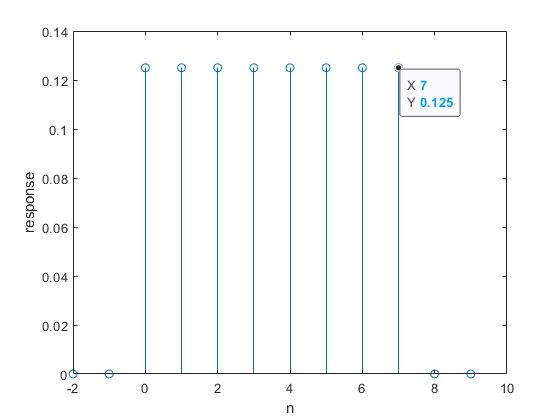
\includegraphics[width=0.6\textwidth]{8.png}
    \caption{Exercise 4, Impulse Response}
    \label{fig:8}
\end{figure}
\subsection{Exercise 5}
The result from the $x[n]$ can be seen as the second plot in figure \ref{fig:4}. The output sequence is the result of convolving the impulse response from $y[n]$, $h[n]$ with $x[n]$ which results in the first plot of figure \ref{fig:4}.


\begin{figure}
    \centering
    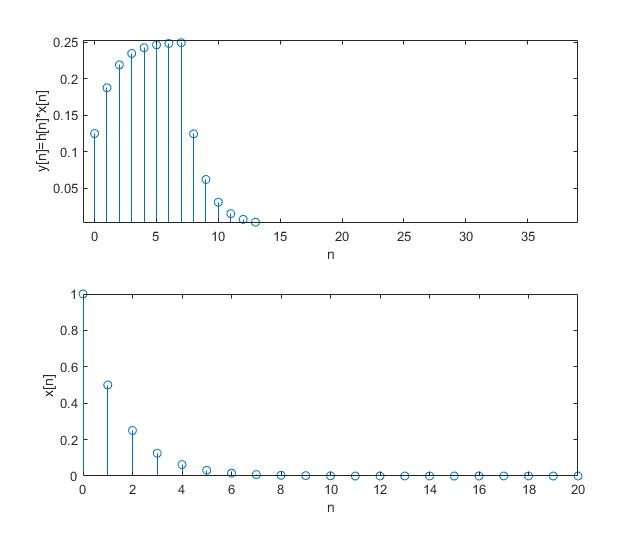
\includegraphics[width=0.6\textwidth]{4.png}
    \caption{Exercise 5, New input signal}
    \label{fig:4}
\end{figure}
\subsection{Exercise 6}
The new output $y[n] = h[n]*x[n+2]$ is shown in figure \ref{fig:5} as the first plot. The input $x[n+2]$ is shown as the second plot.
\begin{figure}
    \centering
    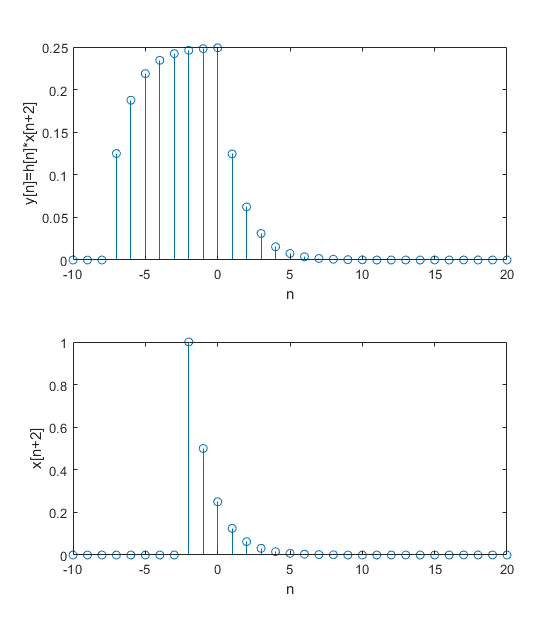
\includegraphics[width=0.6\textwidth]{5.png}
    \caption{Exercise 6, x[n+2]}
    \label{fig:5}
\end{figure}

\subsection{Exercise 7}
The new output $y[n] = h[-n]*x[n]$ is shown in figure \ref{fig:6} as the first plot. The input $x[n]$ is shown as the second plot.
\begin{figure}
    \centering
    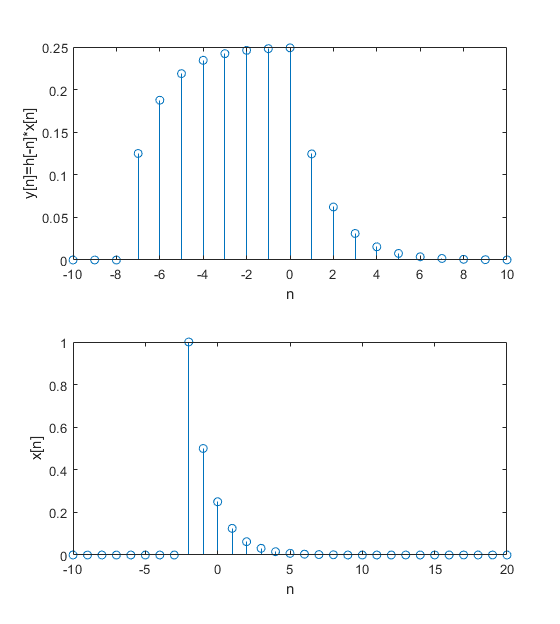
\includegraphics[width=0.6\textwidth]{6.png}
    \caption{Exercise 7, y[n] with h[-n]}
    \label{fig:6}
\end{figure}
\subsection{Exercise 8}
The new output $y[n] = h[h]*x[n]$ with $x[n] = cos(\frac{\pi}{8} \cdot n)+cos(\frac{\pi}{4} \cdot b) , 0 \leq n \leq 127$ is shown in figure \ref{fig:7} as the first plot. The input $x[n]$ is shown as the second plot.
\\
The frequency of the output seems almost like the reverse of the input signal in shape, but not exactly in value. It acts as a sort of compression of the values in the time-frame (the result is $\sim$half as long with same amount of samples), as though it tries to average out the input.
\begin{figure}
    \centering
    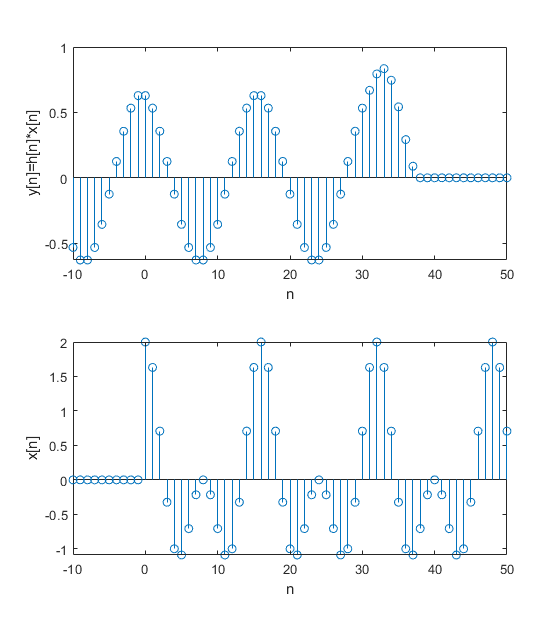
\includegraphics[width=0.6\textwidth]{7.png}
    \caption{Exercise 8, y[n] with h_2[n]}
    \label{fig:7}
\end{figure}
\\
\subsection{Exercise 9}
After processed by the system the audio has a reduced audio quality. The sound has been compressed.
\end{document}
